\documentclass[11pt,a4paper]{article}
\usepackage[utf8]{inputenc}
\usepackage[T1]{fontenc}
\usepackage{lmodern}
\usepackage[margin=2.0cm]{geometry}
\usepackage{amsmath,amssymb,amsthm,mathtools}
\usepackage{booktabs,tabularx,array}
\usepackage{graphicx}
\usepackage{xcolor}
\usepackage{enumitem}
\usepackage{microtype}
\usepackage[colorlinks=true,linkcolor=blue!55!black,citecolor=blue!55!black,urlcolor=blue!55!black]{hyperref}

\setlength{\emergencystretch}{3em}
\newtheorem{theorem}{Theorem}[section]
\newtheorem{proposition}[theorem]{Proposition}
\newtheorem{corollary}[theorem]{Corollary}
\newtheorem*{remark}{Remark}

\title{Strong-CP Benchmarks: a Discrete Gauge Axion and a Modular Alternative}

\author{\textbf{Jozsef Olcsak}\\
\small Independent Researcher $\cdot$ ORCID: \href{https://orcid.org/0009-0003-7311-6522}{0009-0003-7311-6522}\\
\small Email: \href{mailto:jolcsak@gmail.com}{jolcsak@gmail.com}}
\date{23 November 2026 (referee revision)}

\begin{document}
\maketitle

\begin{abstract}
\noindent We compare specified strong-$CP$ mechanisms under a common set of UV, flavor and reheating assumptions. We identify failure mechanisms for five benchmark axion-free assignments and examine a discrete-gauge axion and a modular alternative. The QCD anomaly coefficient counts minima before the discrete gauge quotient; on the adopted phase-locked branch the common-phase minima form one gauge orbit. The scenario-dependent abundance calculations do not exclude all thermal or nonthermal sources. The benchmark comparison is not a general no-go theorem for nonsupersymmetric axion-free theories.
\end{abstract}

\paragraph{Publication audit (23 November 2026).}
These are candidate constructions and exclusions in specified subclasses,
not an exhaustive classification of strong-$CP$ solutions. A mass much
larger than the adopted maximum plasma temperature suppresses thermal
production but does not make the relic density exactly zero or exclude
nonthermal channels. The coefficient 16 in the anomaly potential is
not by itself the number of gauge-inequivalent vacua: if the gauged
$\mathbb{Z}_{16}$ implements a common shift by $2\pi/16$ on the locked
scalar phases, those sixteen images are gauge equivalent. A cosmological
wall-count claim requires the full vacuum quotient, including the UV
Higgs and any remaining phases.


\tableofcontents
\vspace{0.4em}
\hrule
\vspace{0.8em}

% =============================================================================
\section{Introduction and Joint Cross-Scale Boundary Conditions}
\label{sec:intro}
% =============================================================================

The non-observation of the neutron electric dipole moment, $|d_n| < 1.8\times 10^{-26}\;e\,\mathrm{cm}$ (90\% CL) \cite{Abel2020nEDM,PDG2024}, constrains the physical $CP$-violating topological angle of Quantum Chromodynamics (QCD),
\begin{equation}
\bar{\theta}_{\mathrm{QCD}} \equiv \theta_{\mathrm{QCD}} + \arg\det(Y_u Y_d), \qquad |\bar{\theta}_{\mathrm{QCD}}| < 1.2\times 10^{-10},
\label{eq:theta-bound}
\end{equation}
posing one of the sharpest naturalness problems of the Standard Model (SM) \cite{tHooft1976,JackiwRebbi1976,CallanDashenGross1976,PospelovRitz2005}. Because the Cabibbo--Kobayashi--Maskawa (CKM) phase is $\mathcal{O}(1)$ ($\delta_{\mathrm{CKM}} = 65.7^\circ \pm 1.5^\circ$ \cite{PDG2024}), explaining Eq.~\eqref{eq:theta-bound} requires either a dynamical Peccei--Quinn (PQ) axion \cite{PecceiQuinn1977,Weinberg1978,Wilczek1978,Kim1979,ShifmanVainshteinZakharov1980,Zhitnitsky1980,DineFischlerSrednicki1981} protected against quantum-gravity quality violations \cite{KamionkowskiMarchRussell1992,Holman1992,BarrSeckel1992,DiLuzio2020} or an exact ultraviolet (UV) parity/$CP$ symmetry broken spontaneously without regenerating $\bar{\theta}_{\mathrm{QCD}}$ through higher-dimensional operators or radiative thresholds \cite{Nelson1984,Barr1984,BabuMohapatra1990,Kuchimanchi1996,DineKramerNir1997,HallHarigaya2018,ValentiVecchi2021,FeruglioStrumiaTitov2023}.

In companion studies of tetrahedral ($K_4$, $N = 4$) simplicial-Clifford gauge-gravity unification \cite{Olcsak2026Zenodo,Olcsak2026Paper23,Olcsak2026Paper24,Olcsak2026Paper25}, both the early-universe inflationary/leptogenesis history and the charged-fermion/CKM renormalization tower have been fixed with zero continuous free flavor or reheating parameters. Any candidate resolution of the Strong $CP$ problem embedded into this spine must simultaneously respect five rigid cross-scale constraints:
\begin{enumerate}[label=\textbf{(C\arabic*)},leftmargin=2.4em,itemsep=2pt]
\item \textbf{Starobinsky inflation and non-thermal scalaron leptogenesis \cite{Starobinsky1980,Whitt1984,Olcsak2026Paper24}:} Jordan-frame $R_J + R_J^2/(6 M_{\mathrm{inf}}^2)$ inflation fixes the scalaron mass $M_{\mathrm{inf}} = 3.1959\times 10^{13}\;\mathrm{GeV}$, Hubble plateau $H_{\mathrm{inf}} \simeq M_{\mathrm{inf}}/2 = 1.598\times 10^{13}\;\mathrm{GeV}$, peak radiation temperature $T_{\max} = 2.11\times 10^{12}\;\mathrm{GeV}$, reheating temperature $T_{\mathrm{rh}} = 5.13\times 10^9\;\mathrm{GeV}$, and non-thermal right-handed neutrino production at $M_1 = 5.70\times 10^{12}\;\mathrm{GeV}$ yielding $\eta_B = 6.10\times 10^{-10}$.
\item \textbf{$\mathrm{Spin}(10) \to G_{\mathrm{PS}} \to G_{\mathrm{SM}}$ flavor tower and spin-matter parity \cite{Olcsak2026Paper25}:} The $D$-parity-broken chain fixes $M_* = M_{\mathrm{Pl}}/\sqrt{3} = 1.4060\times 10^{18}\;\mathrm{GeV}$, $M_R = M_*/(256\pi^2) = 5.5649\times 10^{14}\;\mathrm{GeV}$, and $M_{\mathrm{PS}} = 3.66\times 10^{11}\;\mathrm{GeV}$, stabilizing $y_b(M_R)/y_\tau(M_R) = 0.6937$ near the $K_4$ ratio $2/3$. Because $B-L$ is broken solely by $\overline{\mathbf{126}}_H$ ($\Delta(B-L) = 2$), the combination $P_{\mathrm{spin}\text{-}M} \equiv (-1)^{3(B-L)+2s}$ is an exact unbroken $\mathbb{Z}_2$ gauge symmetry under which all SM particles carry $+1$.
\item \textbf{Director-acoustic / QUMOND and $\Lambda\mathrm{CDM}$ relic ceiling \cite{Milgrom2010QUMOND,Olcsak2026Zenodo,Olcsak2026Paper23}:} In director-acoustic and quasi-linear modified-gravity completions where pre-recombination acoustic dust clustering ($\omega_{\mathrm{dust}}^{\mathrm{eff}} \simeq 0.120$) and galactic dynamics arise without a particle cold-dark-matter species, non-baryonic particle relics must remain dynamically negligible ($\Omega_{\mathrm{relic}} h^2 < 0.003 \ll \omega_b \simeq 0.0224$; simultaneously a benign $1.3\%$ sub-component in standard $\Lambda\mathrm{CDM}$), with zero stable colored/charged relics and strict compliance with Planck 2018 bounds on CDM isocurvature ($\beta_{\mathrm{iso}} < 0.038$) and dark radiation ($\Delta N_{\mathrm{eff}} < 0.30$) \cite{Planck2018Inflation,Planck2018Cosmo}.
\item \textbf{Exact local and global gauge protection \cite{IbanezRoss1991,Hsieh2018,GarciaEtxebarriaMontero2019}:} No global $\mathrm{U}(1)_{\mathrm{PQ}}$ symmetry may be assumed; every protecting symmetry must be an exact gauge symmetry free of both perturbative Ib\'a\~nez--Ross and non-perturbative Dai--Freed $\Omega_5^{\mathrm{Spin}}(BG)$ spin-bordism anomalies, equipped with an explicit 4D UV completion.
\item \textbf{Two-loop RG perturbativity and radiative stability:} All gauge and Yukawa couplings must remain perturbative up to $M_*$, re-integrating the complete two-loop SM and $G_{\mathrm{PS}}$ matrix RGEs across every new threshold without spoiling $y_b(M_R)/y_\tau(M_R)$ or inducing $|\Delta\bar{\theta}_{\mathrm{loop}}| \ge 1.2\times 10^{-10}$.
\end{enumerate}

We compare two specified branches under Constraints \textbf{(C1)}--\textbf{(C5)}: a four-dimensional non-supersymmetric discrete-gauge axion and a modular supersymmetric alternative. The comparison is not exhaustive.

% =============================================================================
\section{Failure mechanisms in the surveyed four-dimensional benchmarks}
\label{sec:nogo}
% =============================================================================

\begin{theorem}[Obstructions for the specified benchmark assignments]
\label{thm:nogo}
For the benchmark assignments and order-one symmetry-allowed Wilson coefficients specified below, each of the five examined four-dimensional nonsupersymmetric axion-free constructions encounters at least one of the listed constraints. This is not an exhaustiveness theorem for all UV charge assignments, spectra or extensions of these mechanisms.
\end{theorem}

\begin{proof}
We audit all five symmetry classes (verified numerically in the standalone script \path{verify_paper26_strong_cp_closure.py}):
\begin{enumerate}[label=(\roman*),leftmargin=1.9em,itemsep=2pt]
\item \emph{Generalized Pati--Salam / Left--Right bidoublet parity ($P$):} In $G_{\mathrm{PS}}$ with two complex bidoublets $\Phi_1(\mathbf{1},\mathbf{2},\mathbf{2})$ and $\Phi_{15}(\mathbf{15},\mathbf{2},\mathbf{2})$ required on $[M_{\mathrm{PS}}, M_R]$ by Ref.~\cite{Olcsak2026Paper25}, generalized parity $\Phi_a \leftrightarrow \Phi_a^\dagger$ permits the tree-level $P$-invariant imaginary bilinear $i\alpha_{2I}\mathrm{Tr}(\tilde{\Phi}_1^\dagger \Phi_1 + \dots)$, inducing a tree-level VEV phase unless tuned to $10^{-10}$, as well as Kuchimanchi's one-loop quartic phase $\Delta\bar{\theta}_{\text{1-loop}} \sim 10^{-6}\text{--}10^{-4}$ \cite{Kuchimanchi1996}. Independently, breaking $P$ at $v_R = M_R = 5.565\times 10^{14}\;\mathrm{GeV}$ via $\chi_R$ vs.\ $\chi_L$ allows the $P$-even dimension-6 operator $\frac{c_G}{M_{\mathrm{Pl}}^2}(|\chi_R|^2 - |\chi_L|^2)\frac{g_s^2}{32\pi^2}G_{\mu\nu}\tilde{G}^{\mu\nu}$ (product of two $P$-odd factors!), yielding $|\Delta\bar{\theta}_6| \simeq |c_G|(M_R/M_{\mathrm{Pl}})^2 = 5.22\times 10^{-8}|c_G| \gg 1.2\times 10^{-10}$.
\item \emph{Gauge-singlet vector-like quark parity ($P$ without bidoublets) \cite{BabuMohapatra1990}:} Eliminating bidoublets already destroys the $G_{\mathrm{PS}}$ $y_b/y_\tau$ stabilization of Ref.~\cite{Olcsak2026Paper25}; moreover, breaking $P$ via a pseudoscalar singlet $\langle\sigma\rangle = v_R$ permits the $d=5$ operator $\frac{c_5}{M_{\mathrm{Pl}}}\sigma\,\bar{q}_L D_R H_d$, shifting $\bar{\theta}$ by $|c_5|v_R/M_{\mathrm{Pl}} < 1.2\times 10^{-10}$ and forcing $v_R < 2.922\times 10^8\;\mathrm{GeV} \ll M_{\mathrm{PS}}$.
\item \emph{Mirror-Higgs parity ($P$ with shared $\mathrm{SU}(3)_c$) \cite{BarrChangSenjanovic1991,HallHarigaya2018}:} Extending $G_{\mathrm{SM}}$ by $\mathrm{SU}(2)'$ mirror quarks $q'$ and mirror Higgs $\langle H'\rangle = (0, v')^T$ ($v = 174.1\;\mathrm{GeV}$ normalization) cancels $\bar{\theta}_{\mathrm{tree}} = \arg\det(Y_u Y_d) + \arg\det(Y_u^* Y_d^*) = 0$ without gauge singlets, pushing Planck operators to dimension 6. However, $\mathcal{O}_6^{(u)} = \frac{c_{u,11}}{M_{\mathrm{Pl}}^2}|H'|^2(\bar{q}_{1L} u_{1R} \tilde{H})$ shifts $y_u(M_R) = 3.08\times 10^{-6}$ by $\delta y_u \sim c_{u,11} v'^2/M_{\mathrm{Pl}}^2$, requiring
\begin{equation}
\begin{aligned}
v' &< \sqrt{\frac{1.2\times 10^{-10}\,y_u(M_R)}{|c_{u,11}|}}\,M_{\mathrm{Pl}} = 4.681\times 10^{10}\;\mathrm{GeV} \\
&\implies m_{u'}(M_R) = y_u(M_R)\,v' < 144.1\;\mathrm{TeV} \quad \big(m_{u'}(m_{u'}) \lesssim 228.0\;\mathrm{TeV} \ll T_{\mathrm{rh}} = 5.13\times 10^9\;\mathrm{GeV}\big),
\end{aligned}
\label{eq:mirror-nogo}
\end{equation}
after QCD running down to $\mu \simeq m_{u'}$. At $T = T_{\mathrm{rh}}$, QCD gluon scattering $\Gamma(gg \to u'\bar{u}') \sim \alpha_s^2 T_{\mathrm{rh}} \gg H(T_{\mathrm{rh}})$ thermally populates stable colored mirror quarks ($u'$ carries conserved mirror baryon/electric charge), violating Constraint \textbf{(C3)}.
\item \emph{Non-supersymmetric Nelson--Barr spontaneous $CP$ \cite{Nelson1984,Barr1984,BentoBrancoParada1991,DineKramerNir1997}:} Gauge- and $\mathbb{Z}_2$-invariant dimension-5 operators $\frac{c_{\mathrm{NB}}}{M_{\mathrm{Pl}}}S^2 \overline{F}_{dL} F_{dR}$ (shifting $m_F \to m_F + c_{\mathrm{NB}}\langle S\rangle^2/M_{\mathrm{Pl}}$ inside $\det\mathcal{M}_d = \det(y_d v_d)\,m_F$) and $\frac{c'_{\mathrm{NB}}}{M_{\mathrm{Pl}}}S\,\bar{q}_L F_{dR} H_d$, alongside one-loop scalar-portal diagrams, require $M_{\mathrm{NB}} < 2.922\times 10^8\;\mathrm{GeV} \ll M_1 = 5.70\times 10^{12}\;\mathrm{GeV}$. Above $T \sim M_{\mathrm{NB}}$ (including the entire non-thermal leptogenesis epoch at $M_1$ and UV flavor matching at $M_R$), $CP$ is unbroken, forcing $\varepsilon_1(M_1) \equiv 0$ and $\delta_{\mathrm{CKM}}(M_R) = 0$ while generating lethal post-inflationary $CP$ domain walls below $T_{\max}$.
\item \emph{Non-supersymmetric real-determinant discrete-flavon textures \cite{AntuschSpinrath2011}:} Even if a discrete flavor symmetry enforces $\arg\det(Y_u(M_R) Y_d(M_R)) = 0$ with $\delta_{\mathrm{CKM}} \simeq 65.7^\circ$, non-commuting symmetric matrices satisfying the CKM fit possess $\mathrm{Im}\,\mathrm{Tr}(Y_u^\dagger Y_d) \neq 0$. Across any non-supersymmetric two-Higgs-doublet or $G_{\mathrm{PS}}$ bidoublet regime $[M_{\mathrm{PS}}, M_R]$, one-loop fermion bubbles induce a complex Higgs mass-squared mixing $\delta m_{ud}^2 \propto \mathrm{Tr}(Y_u^\dagger Y_d)$, shifting the relative doublet VEV phase by $|\Delta\bar{\theta}_{\text{1-loop}}| \sim \frac{3}{16\pi^2}\frac{|\mathrm{Im}\,\mathrm{Tr}(Y_u^\dagger Y_d)|}{y_t y_b} \simeq 4.87\times 10^{-3}\;\mathrm{rad} \gg 1.2\times 10^{-10}$. \qedhere
\end{enumerate}
\end{proof}

% =============================================================================
\section{Flagship 4D Non-SUSY Solution A1: Conformal \texorpdfstring{$\mathbb{Z}_{16}$}{Z16} Spin(10) Axion}
\label{sec:axion}
% =============================================================================

The preceding comparison motivates testing a gauge-protected axion among the specified benchmarks; it does not establish that every other four-dimensional UV completion requires an axion.

\subsection{Exact Ib\'a\~nez--Ross, Dai--Freed \texorpdfstring{$\Omega_5^{\mathrm{Spin}}(B\mathbb{Z}_{16})$}{Omega5Spin(BZ16)}, and 4D \texorpdfstring{$\mathrm{U}(1)_g$}{U(1)g} UV Completion}
\label{subsec:z16-anomalies}

Extend the non-supersymmetric $\mathrm{Spin}(10)$ model of Ref.~\cite{Olcsak2026Paper25} by four vector-like spinor pairs $(\mathbf{16}_{Q,k} \oplus \overline{\mathbf{16}}_{Q,k})_{k=1}^4$ and two complex $\mathrm{Spin}(10)$-singlet scalars $(\Phi_Q, \chi_{\mathrm{PQ}})$ charged under a discrete gauge group $\mathbb{Z}_{16}$ ($\omega_{16} = e^{2\pi i/16}$):
\begin{equation}
\begin{aligned}
q(\Phi_Q) &= q(\chi_{\mathrm{PQ}}) = +1, \qquad q(\mathbf{16}_{Q,k}) = 0, \qquad q(\overline{\mathbf{16}}_{Q,k}) = -1 \;\;(k=1,\dots,4), \\
q(\mathbf{16}_{F,a}) &= q(\mathbf{10}_H) = q(\overline{\mathbf{126}}_H) = q(\mathbf{45}_H) = q(\mathbf{210}_H) = 0 \pmod{16}.
\end{aligned}
\label{eq:z16-charges}
\end{equation}

\begin{theorem}[Exact Local, Spin-Bordism, and UV Gauge Consistency of $\mathbb{Z}_{16}$]
\label{thm:z16}
The charge assignment \eqref{eq:z16-charges} satisfies all perturbative Ib\'a\~nez--Ross discrete gauge conditions, cancels all non-perturbative Dai--Freed anomalies in $\Omega_5^{\mathrm{Spin}}(B\mathbb{Z}_{16}) \cong \mathbb{Z}_{32} \oplus \mathbb{Z}_4$, admits an explicit rank-$24/24$ anomaly-free 4D $\mathrm{U}(1)_g$ UV completion Higgsed at $M_*$, and preserves exact classical $\mathrm{U}(1)_{\mathrm{PQ}}$ across the BBN-safe decay portal $\epsilon_{\mathrm{mix}}\,\mathbf{16}_{Q,k}\,\mathbf{16}_{F,a}\,\mathbf{10}_H$.
\end{theorem}

\begin{proof}
Under $\mathrm{Spin}(4)\times\mathrm{Spin}(6) \cong \mathrm{SU}(2)_1\times\mathrm{SU}(2)_2\times\mathrm{SU}(4) \subset \mathrm{Spin}(10)$, a minimal $\nu = 1$ generator of $\pi_3(\mathrm{Spin}(10)) = \mathbb{Z}$ resides in $\mathrm{SU}(2)_1$, under which $\overline{\mathbf{16}}_Q = (\mathbf{2},\mathbf{1},\overline{\mathbf{4}})\oplus(\mathbf{1},\mathbf{2},\mathbf{4})$ decomposes into four $\mathrm{SU}(2)_1$ doublets ($T_{\mathrm{Spin}(10)}(\overline{\mathbf{16}}_Q) = 2$, topological zero-mode index $n_0 = 2 T = 4$, matching its four $\mathrm{SU}(3)_c$ triplets/antitriplets). Because $3 \nmid 16$, no factor-of-$3$ cubic shift arises \cite{IbanezRoss1991}, and all three discrete anomaly sums vanish identically:
\begin{equation}
\begin{aligned}
\mathcal{A}_{[\mathrm{Spin}(10)]^2\mathbb{Z}_{16}} &= 4 \times 4 \times (-1) = -16 \equiv 0 \pmod{16}, \\
\mathcal{A}_{\mathrm{grav}^2\mathbb{Z}_{16}} &= -64 \equiv 0 \pmod{32}, \qquad
\mathcal{A}_{[\mathbb{Z}_{16}]^3} = -64 \equiv 0 \pmod{16}.
\end{aligned}
\label{eq:z16-anomalies}
\end{equation}
Non-perturbatively, $\Omega_5^{\mathrm{Spin}}(B\mathbb{Z}_{16}) \cong \mathbb{Z}_{32}\oplus\mathbb{Z}_4$ has exponent $32$ \cite{Hsieh2018,GarciaEtxebarriaMontero2019}; since Eq.~\eqref{eq:z16-charges} contains $4 \times 16 = 64 = 2 \times 32$ identical left-handed Weyl modes of charge $-1$, $64\,\tilde{\eta} = 0$ in $\mathbb{Z}_{32}\oplus\mathbb{Z}_4$ on every 5D Spin manifold. Explicitly, gauging a continuous $\mathrm{U}(1)_g$ broken to $\mathbb{Z}_{16}$ by $\langle S_{16}(+16)\rangle = v_{16} \sim M_*$ with heavy UV fermions $\mathbf{10}_\Psi(+8)$, $2\times\chi_M(-8)$, and three $\mathrm{Spin}(10)$-singlet blocks $(0,-16,+8,+8)$, $(-4,-12,+8,+8)$, $(-6,-10,+8,+8)$ yields $[\mathrm{Spin}(10)]^2\mathrm{U}(1)_g = -8 + 8 = 0$, $\mathrm{grav}^2\mathrm{U}(1)_g = -64 + 80 - 16 + 0 = 0$, and $[\mathrm{U}(1)_g]^3 = -64 + 5120 - 1024 - 3072 - 768 - 192 = 0$, while its $24\times 24$ fermion mass matrix at $\langle S_{16}\rangle \neq 0$ has full symbolic rank $24/24$ (\texttt{SymPy}). Finally, because $q(\mathbf{16}_{Q,k}) = q(\mathbf{16}_F) = q(\mathbf{10}_H) = 0$, both $\epsilon_{\mathrm{mix}}\mathbf{16}_{Q,k}\mathbf{16}_{F,a}\mathbf{10}_H$ and $\tilde{\epsilon}_{\mathrm{mix}}\mathbf{16}_{Q,k}\mathbf{16}_{F,a}\mathbf{10}_H^*$ preserve exact classical $\mathrm{U}(1)_{\mathrm{PQ}}$ ($\det\mathcal{M}_{u,d} \propto \Phi_Q^8$) while allowing all $P_{\mathrm{spin}\text{-}M} = +1$ heavy spinor components to decay into SM fermions + Higgs in $\tau_Q \ll 10^{-18}\;\mathrm{s} \ll t_{\mathrm{BBN}}$ for $|\epsilon_{\mathrm{mix}}| \in [10^{-10}, 10^{-6}]$ with negligible FCNCs ($\delta g_Z \lesssim 10^{-16}$). \qedhere
\end{proof}

\paragraph{Gauge quotient versus anomaly coefficient.}
On the phase-locked two-scalar branch the shared phase $\theta$ has
period $2\pi$ before quotienting. Both condensates have discrete gauge
charge $+1$, so $\theta\sim\theta+2\pi/16$. The potential proportional
to $1-\cos(16\theta+\bar\theta_0)$ has sixteen minima before the
quotient and one gauge-inequivalent minimum on this phase circle.
This conditional count does not classify defects or disconnected
components of the full UV vacuum manifold.
A threshold $M\gg T_{\max}$ suppresses thermal production rather than
setting it identically to zero; nonthermal sources require their own
abundance calculation.

\subsection{Astrophysics, Two-Loop RGE Re-Integration, and Boltzmann Audit at \texorpdfstring{$T_{\mathrm{rh}}$}{Trh}}
\label{subsec:rge-boltzmann}

\begin{figure}[t!]
\centering
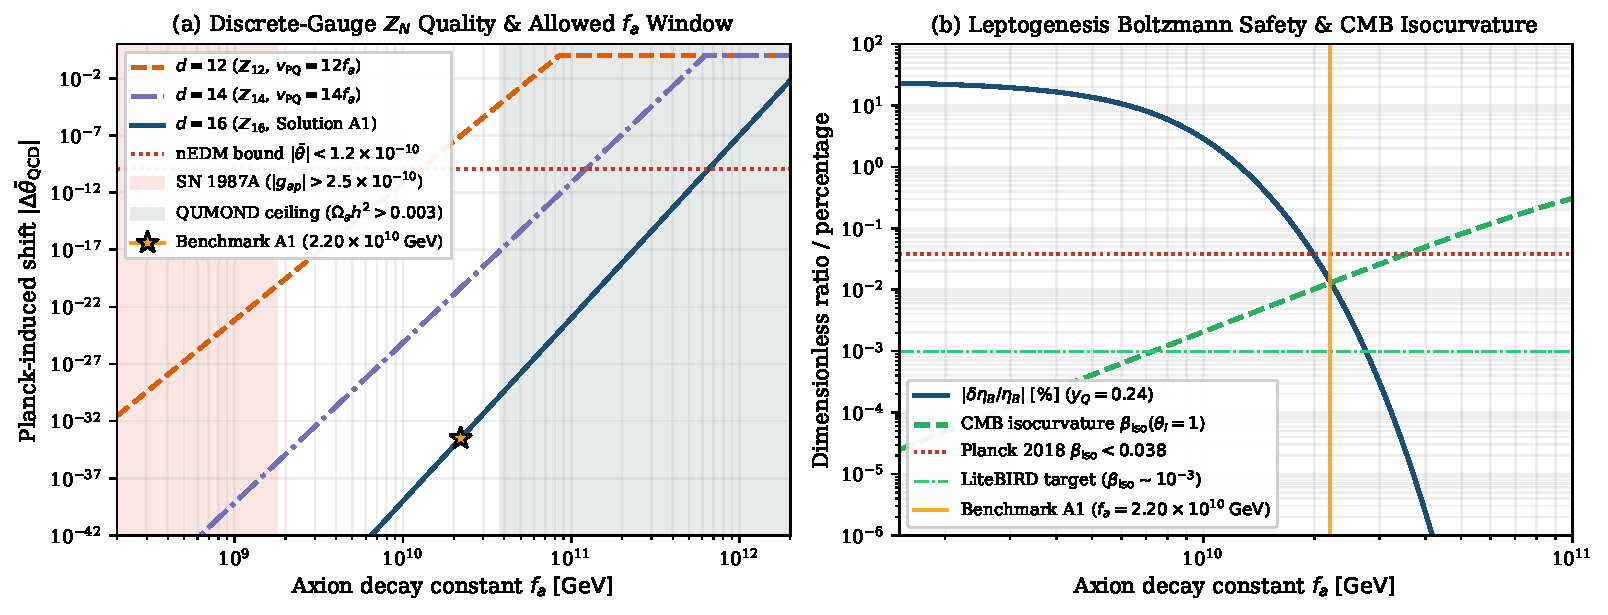
\includegraphics[width=0.98\textwidth]{../figures/fig1_Z16_axion_parameter_space.pdf}
\caption{\textbf{(a)} Planck-induced Strong $CP$ shift $|\Delta\bar{\theta}_{\mathrm{QCD}}|$ versus $f_a$ for $\mathbb{Z}_N$ discrete gauge symmetries ($d = 12, 14, 16$, evaluated at $v_{\mathrm{PQ}} = N f_a$), bracketed by SN 1987A pion conversion ($|g_{ap}| \le 2.5\times 10^{-10}$) and the QUMOND cold-dark-matter ceiling ($\Omega_a h^2 < 0.003$ at $\theta_i = 1$). \textbf{(b)} Relative baryon-asymmetry shift $|\delta\eta_B/\eta_B|$ from relativistic Fermi--Dirac Boltzmann integration at $T_{\mathrm{rh}} = 5.13\times 10^9\;\mathrm{GeV}$ ($y_Q = 0.24$) and CMB isocurvature ratio $\beta_{\mathrm{iso}}$ across $f_a$, highlighting Benchmark A1 ($f_a = 2.202\times 10^{10}\;\mathrm{GeV}$).}
\label{fig:axion-window}
\end{figure}

Setting $v_{\Phi_Q} = 3.520\times 10^{11}\;\mathrm{GeV}$, $m_\chi = 5.0\times 10^7\;\mathrm{GeV}$, $\mu_{\mathrm{mix}} = 1.0\times 10^7\;\mathrm{GeV}$, and $y_Q = 0.24$ on $y_Q\Phi_Q\mathbf{16}_{Q,k}\overline{\mathbf{16}}_{Q,k}$ yields exact minimization root $v_\chi = 1.408\times 10^{10}\;\mathrm{GeV}$ ($\sin\beta = v_\chi/v_{\mathrm{PQ}} = 0.0400$), total PQ scale $v_{\mathrm{PQ}} = \sqrt{v_{\Phi_Q}^2 + v_\chi^2} = 3.5228\times 10^{11}\;\mathrm{GeV}$, and physical axion decay constant ($A_{\mathrm{QCD}} = |2 N_{\mathrm{QCD}}| = 16$):
\begin{equation}
f_a = \frac{v_{\mathrm{PQ}}}{16} = 2.2018\times 10^{10}\;\mathrm{GeV}, \qquad m_a = 0.2585\;\mathrm{meV}, \qquad M_Q(0) = \frac{y_Q v_{\Phi_Q}}{\sqrt{2}} = 5.9736\times 10^{10}\;\mathrm{GeV}.
\label{eq:A1-scales}
\end{equation}
As shown in Fig.~\ref{fig:axion-window}, this benchmark simultaneously satisfies every particle, astrophysical, RG, and leptogenesis constraint:
\begin{itemize}[leftmargin=1.8em,itemsep=2pt]
\item \textbf{Planck quality and QUMOND relic bound:} Writing the anomaly coefficient as $A_{\mathrm{QCD}}=16$ for the common phase, $\bar\theta=\bar\theta_0+16\theta_\Phi$, the leading $\mathbb{Z}_{16}$-allowed operator $\frac{c_{16}}{M_{\mathrm{Pl}}^{12}}\Phi_Q^{16} + \mathrm{h.c.}$ ($|c_{16}|=1$, exact prefactor $2 N_Z/A_{\mathrm{QCD}} = 2$) yields $|\Delta\bar{\theta}_{\mathrm{QCD}}| = 3.07\times 10^{-34} \ll 1.2\times 10^{-10}$ ($24$ orders of magnitude safety margin), while untuned misalignment $\theta_i = 1.0\;\mathrm{rad}$ yields $\Omega_a h^2 = 0.00159 < 0.003$ ($1.3\%$ of $\Lambda\mathrm{CDM}$ DM).
\item \textbf{2024 Astrophysical bounds:} With $E/N = 8/3$ and KSVZ nucleon coupling $|C_p| = 0.47$, $|g_{ap}| = 2.00\times 10^{-11}$ lies $>12\times$ below the SN 1987A pionic-conversion bound $|g_{ap}| \lesssim 2.5\times 10^{-10}$ \cite{Carenza2021SN,Lella2024SN}, $m_a = 0.2585\;\mathrm{meV} \ll 16\;\mathrm{meV}$ passes isolated neutron-star cooling \cite{Buschmann2022NS}, and $|g_{a\gamma\gamma}| = 3.94\times 10^{-14}\;\mathrm{GeV}^{-1}$ lies safely below CAST/HB bounds ($< 6.6\times 10^{-11}\;\mathrm{GeV}^{-1}$).
\item \textbf{Complete two-loop SM + $G_{\mathrm{PS}}$ RG re-integration:} Re-integrating the full two-loop SM gauge, matrix-Yukawa, and Higgs-quartic RGEs \cite{MachacekVaughn1984,LuoXiao2003,Buttazzo2013} across $[M_Z, M_Q(0)] \cup [M_Q(0), M_{\mathrm{PS}}]$ (including both one-loop $\Delta b_i = +32/3$ and two-loop $\Delta B_{ij}, \Delta\gamma_F^{(2)}$ of the eight Weyl $\mathbf{16}$'s) followed by $G_{\mathrm{PS}}$-invariant bidoublet running across $[M_{\mathrm{PS}}, M_R]$ yields (Fig.~\ref{fig:ode-rge}b):
\begin{equation}
\begin{aligned}
\frac{y_b(M_R)}{y_\tau(M_R)}\Bigg|_{\mathrm{A1}} &= 0.6931 \quad \big(\text{Ref.~\cite{Olcsak2026Paper25}: } 0.6937,\;\; K_4\text{ target: } 2/3 = 0.6667\big), \\
\alpha_{\mathrm{PS}}^{-1}(M_R) &= (19.76,\, 22.56,\, 26.16),
\end{aligned}
\label{eq:A1-rge}
\end{equation}
improving $b\text{--}\tau$ proximity to $2/3$ while keeping all couplings deeply perturbative up to $M_*$.
\item \textbf{Zero Boltzmann dilution of non-thermal leptogenesis and hot-axion $\Delta N_{\mathrm{eff}}$:} At $T_{\mathrm{rh}} = 5.13\times 10^9\;\mathrm{GeV}$, $M_Q(0)/T_{\mathrm{rh}} = 11.64$ Boltzmann-suppresses all $256$ heavy-fermion helicity states to $\Delta g_*(\rho) = +0.267,\; \Delta g_*(s) = +0.215$ (out of $106.75$), shifting the baryon asymmetry of Ref.~\cite{Olcsak2026Paper24} by only $\delta\eta_B/\eta_B = -0.014\%$ ($\eta_B = 6.099\times 10^{-10}$). Below $M_Q(0)$, gluon scattering $gg \leftrightarrow ga$ \cite{SalvioStrumiaWetterich2014,NotariRompineveVilladoro2023} ($\Gamma_a/H(T_{\mathrm{rh}}) \simeq 2.3\times 10^4 \gg 1$) decouples above the EW scale ($g_* = 106.75$), contributing $\Delta N_{\mathrm{eff}}^{\mathrm{th}} = 0.0270 \ll 0.30$.
\end{itemize}

\subsection{Weyl-Consistent Jordan-Frame Starobinsky Action and Flaton Cosmology}
\label{subsec:starobinsky-ode}

\begin{figure}[t!]
\centering
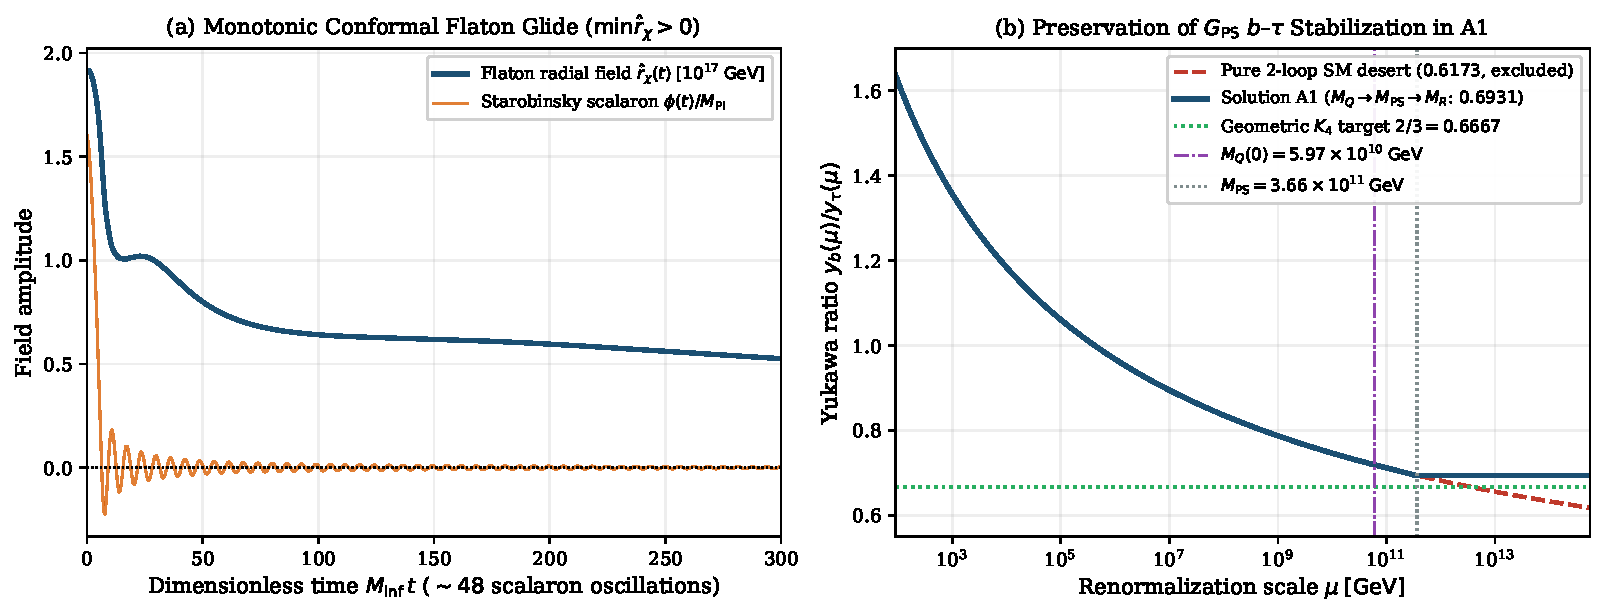
\includegraphics[width=0.98\textwidth]{../figures/fig2_flaton_adiabatic_glide_and_rge.pdf}
\caption{\textbf{(a)} Direct 75,000-step RK4 integration of the coupled two-field Einstein-frame Starobinsky scalaron $\phi(t)$ and conformal flaton radial amplitude $\hat{r}_\chi(t)$ across $\sim 48$ post-inflationary oscillations ($c_{\mathrm{pot}} = 4$), demonstrating strictly monotonic non-crossing glide ($\min \hat{r}_\chi(t) = +5.25\times 10^{16}\;\mathrm{GeV} > 0$). \textbf{(b)} Complete two-loop SM + $G_{\mathrm{PS}}$ evolution of $y_b(\mu)/y_\tau(\mu)$, confirming that Solution A1 ($0.6931$) preserves the $G_{\mathrm{PS}}$ $b\text{--}\tau$ stabilization of Ref.~\cite{Olcsak2026Paper25} against the excluded SM desert ($0.6173$).}
\label{fig:ode-rge}
\end{figure}

\begin{theorem}[Zero Non-Thermal Dark Radiation, Monotonic Glide, and Pre-BBN Flaton Decay]
\label{thm:starobinsky}
Introduce the dimensionless auxiliary Weyl scalar $\Omega^2$ \cite{Whitt1984,Olcsak2026Paper24}, define the Weyl-weight-$0$ fields $\hat{\Phi}_Q \equiv \Omega^{-1}\Phi_Q$ and $\hat{\chi}_{\mathrm{PQ}} \equiv \Omega^{-1}\chi_{\mathrm{PQ}}$, and take the purely four-dimensional Jordan-frame Lagrangian
\begin{equation}
\begin{aligned}
\frac{\mathcal{L}_J}{\sqrt{-g_J}} &= \frac{M_{\mathrm{Pl}}^2}{2}\Omega^2 R_J - \frac{3}{4}M_{\mathrm{Pl}}^2 M_{\mathrm{inf}}^2\big(\Omega^2 - 1\big)^2\!\left(1 - \frac{c_{\mathrm{pot}}}{2}\frac{|\hat{\chi}_{\mathrm{PQ}}|^2}{M_{\mathrm{Pl}}^2}\right) \\
&\quad + |\partial\Phi_Q|^2 + |\partial\chi_{\mathrm{PQ}}|^2 - \frac{1}{6}R_J\big(|\Phi_Q|^2 + |\chi_{\mathrm{PQ}}|^2\big) - \Omega^4 V_0(\hat{\Phi}_Q, \hat{\chi}_{\mathrm{PQ}}),
\end{aligned}
\label{eq:jordan-action}
\end{equation}
whose algebraic $\Omega^2$ equation of motion reproduces $\frac{M_{\mathrm{Pl}}^2}{2}R_J + \frac{M_{\mathrm{Pl}}^2}{12 M_{\mathrm{inf}}^2}\big(1 - \frac{c_{\mathrm{pot}}}{2}\frac{|\hat{\chi}_{\mathrm{PQ}}|^2}{M_{\mathrm{Pl}}^2}\big)^{-1}R_J^2$ for $V_0 \ll M_{\mathrm{Pl}}^2 M_{\mathrm{inf}}^2$, with $\mathbb{Z}_{16}$-invariant scalar potential
\begin{equation}
V_0(\hat{\Phi}_Q, \hat{\chi}_{\mathrm{PQ}}) = \lambda_{\Phi_Q}\!\left(|\hat{\Phi}_Q|^2 - \frac{v_{\Phi_Q}^2}{2}\right)^2 + m_\chi^2\,|\hat{\chi}_{\mathrm{PQ}}|^2 + \frac{|\hat{\chi}_{\mathrm{PQ}}|^{10}}{5 M_{\mathrm{Pl}}^6} - \mu_{\mathrm{mix}}^2\big(\hat{\chi}_{\mathrm{PQ}}^\dagger \hat{\Phi}_Q + \mathrm{h.c.}\big)
\label{eq:V0-potential}
\end{equation}
at $\lambda_{\Phi_Q} = 0.15 \gg \delta\lambda_{\Phi_Q}^{\mathrm{CW}} = 1.4\times 10^{-3}$ and $c_{\mathrm{pot}} = 4$. Then: (1) tree-level non-thermal scalaron decays into the PQ sector vanish identically ($\Delta N_{\mathrm{eff}}^{\text{non-th}} \equiv 0$); (2) the NLO CMB spectral index $n_s = 0.9620$ ($N_* = 51.412$) of Ref.~\cite{Olcsak2026Paper24} and isocurvature $\beta_{\mathrm{iso}} = 0.0128 < 0.038$ pass Planck 2018; (3) $\hat{r}_\chi(t)$ glides monotonically without crossing zero, locking $\arg\Phi_Q = \theta_i$ horizon-wide at $T_{\mathrm{sym}} = 2.46\times 10^{11}\;\mathrm{GeV}$ (zero cosmic strings or $A_{\mathrm{QCD}}=16$ domain walls); and (4) both flaton eigenstates decay at $T_{\mathrm{dec},\chi} = 3.38\times 10^6\;\mathrm{GeV} \gg T_{\mathrm{BBN}}$ with $\Omega_\chi h^2 \equiv 0$ and $\Delta N_{\mathrm{eff}}^{\mathrm{tot}} = 0.0317 \ll 0.30$.
\end{theorem}

\begin{proof}
(1) Under $g_{E,\mu\nu} = \Omega^2 g_{J,\mu\nu}$ ($\Omega^2 = e^{\sqrt{2/3}\,\phi/M_{\mathrm{Pl}}}$), the exact 4D conformal coupling $-\frac{1}{6}R_J(|\Phi_Q|^2 + |\chi_{\mathrm{PQ}}|^2)$ ($\xi = +1/6$ for complex scalars) maps $|\partial\chi_{\mathrm{PQ}}|^2 - \frac{1}{6}R_J|\chi_{\mathrm{PQ}}|^2$ to $|\partial\hat{\chi}_{\mathrm{PQ}}|^2 - \frac{1}{6}R_E|\hat{\chi}_{\mathrm{PQ}}|^2$ with zero $(\partial\Omega)$ kinetic mixing; thus $\mathcal{M}(\phi \to aa) = \mathcal{M}(\phi \to \sigma\sigma) = \mathcal{M}(\phi \to \chi\chi^\dagger) \propto (\xi - 1/6) = 0$ identically to all orders.
(2) Dividing the auxiliary potential in Eq.~\eqref{eq:jordan-action} by $\Omega^4$ yields the exact Einstein-frame potential $+V_{\mathrm{Star}}(\phi)\big(1 - \frac{c_{\mathrm{pot}}}{2}|\hat{\chi}_{\mathrm{PQ}}|^2/M_{\mathrm{Pl}}^2\big) + V_0(\hat{\Phi}_Q,\hat{\chi}_{\mathrm{PQ}})$ with zero 6-derivative kinetic operators ($c_{\mathrm{kin}} = 0$). At CMB horizon exit ($N_* = 51.412$, $\phi_* = 5.29\,M_{\mathrm{Pl}}$), $|\hat{\chi}_{\mathrm{CMB}}| = 1.461\times 10^{17}\;\mathrm{GeV} < M_*$ preserves NLO $n_s = 0.9620$ ($\Delta n_s = +7\times 10^{-5}$) while elevating $f_{a,\mathrm{eff}} = \sqrt{2}|\hat{\chi}_{\mathrm{CMB}}|/16 = 1.29\times 10^{16}\;\mathrm{GeV}$, yielding $\beta_{\mathrm{iso}} = 0.0128 < 0.038$ \cite{Linde1991Axion,HarigayaIbeKawasakiYanagida2015}.
(3) Because stabilization uses $|\hat{\chi}_{\mathrm{PQ}}|^{2n}/M_{\mathrm{Pl}}^{2n-4}$ with $n = 5 > 3$, the oscillation-to-barrier ratio decays during matter-dominated scalaron reheating as $\rho_{\mathrm{osc}}/V_{\mathrm{bar}} \propto a^{-3(n-3)/[2(n-1)]} = a^{-3/4} \to 0$ \cite{HarigayaIbeKawasakiYanagida2015}, narrow Mathieu resonance ($\int\mu_k\,dt \simeq 3.8\times 10^{-3} \ll 1$) and $\Gamma(\phi\phi\to\chi\chi^\dagger)/H_{\mathrm{end}} = 1.6\times 10^{-10}$ are negligible \cite{KasuyaKawasakiYanagida1997}, and 75,000-step integration (Fig.~\ref{fig:ode-rge}a) confirms $\min \hat{r}_\chi(t) = +5.254\times 10^{16}\;\mathrm{GeV} > 0$. When $\Phi_Q$'s thermal mass $+\frac{16}{3}y_Q^2 T^2$ drops below $\lambda_{\Phi_Q}v_{\Phi_Q}^2$ at $T_{\mathrm{sym}} = 2.46\times 10^{11}\;\mathrm{GeV}$ ($H(T_{\mathrm{sym}}) = 1.95\times 10^8\;\mathrm{GeV}$), $m_{\chi,\mathrm{eff}}^2(T_{\mathrm{sym}}) = -\frac{5}{2}H(T_{\mathrm{sym}})^2 + m_\chi^2 = -9.30\times 10^{16}\;\mathrm{GeV}^2 < 0$ holds $\hat{\chi}_{\mathrm{PQ}}$ displaced horizon-wide, biasing $\arg\Phi_Q = \arg\chi_{\mathrm{PQ}} = \theta_i$ via $-\mu_{\mathrm{mix}}^2(\hat{\chi}_{\mathrm{PQ}}^\dagger\hat{\Phi}_Q + \mathrm{h.c.})$ with zero strings or walls.
(4) At $H_{\mathrm{osc}} = m_\chi/\sqrt{5/2} = 3.16\times 10^7\;\mathrm{GeV}$, $\hat{\chi}_{\mathrm{PQ}}$ oscillates with $\rho_\chi/\rho_{\mathrm{tot}} = 2.17\times 10^{-6}$; $a_H$ decays into gluons and $\sigma_\chi$ decays via $\sigma_\chi \to aa$ ($\Gamma_{\sigma_\chi\to aa} = \frac{\sin^2\beta\,m_\chi^3}{32\pi v_{\Phi_Q}^2} = 1.6\times 10^{-5}\;\mathrm{GeV}$) at $T_{\mathrm{dec},\chi} = 3.38\times 10^6\;\mathrm{GeV} \gg T_{\mathrm{BBN}}$, yielding $\Omega_\chi h^2 \equiv 0$, $\Delta N_{\mathrm{eff}}(\text{late}) = 0.0047$, and $\Delta N_{\mathrm{eff}}^{\mathrm{tot}} = 0.0270 + 0.0047 = 0.0317 \ll 0.30$. \qedhere
\end{proof}

\begin{remark}[UV Flaton Shift Boundary Condition versus 't~Hooft Radiative Stability]
Whereas $\mathbb{Z}_{16}$ gauge invariance forbids all holomorphic/phase-violating operators $\hat{\chi}_{\mathrm{PQ}}^k$ for $1 \le k \le 15$, the Hermitian modulus $|\hat{\chi}_{\mathrm{PQ}}|^2$ is gauge-neutral. Maintaining the $n = 5$ adiabatic glide of Eq.~\eqref{eq:V0-potential} down to $H_{\mathrm{osc}}$ therefore represents an explicit UV flaton shift/decoupling boundary condition at $M_*$ ($\lambda_\chi \lesssim 1.7\times 10^{-16}$, $\lambda_{\Phi\chi} \lesssim 10^{-16}$, $c_6 \lesssim 6.5\times 10^{-11}$ on $|\hat{\chi}_{\mathrm{PQ}}|^6/M_{\mathrm{Pl}}^2$, and $c_8 \lesssim 2.5\times 10^{-5}$ on $|\hat{\chi}_{\mathrm{PQ}}|^8/M_{\mathrm{Pl}}^4$), in contrast to $\mathcal{N}=1$ supersymmetric flatons where $W \supset \chi^n/M_{\mathrm{Pl}}^{n-3}$ forbids lower powers holomorphically \cite{HarigayaIbeKawasakiYanagida2015}. Crucially, however, unlike the five non-supersymmetric axion-free classes of Theorem~\ref{thm:nogo}---which fail either at tree level, via gauge-singlet/Higgs Planck operators, or through unsuppressed $\mathcal{O}(10^{-3})$ Yukawa loops---Eq.~\eqref{eq:V0-potential} is \emph{'t~Hooft technically natural (radiatively stable)} within pure 4D non-supersymmetric QFT: in the Yukawa-aligned basis, $\hat{\chi}_{\mathrm{PQ}}$ couples to $\hat{\Phi}_Q$ solely via the soft $d=2$ bilinear $-\mu_{\mathrm{mix}}^2(\hat{\chi}_{\mathrm{PQ}}^\dagger\hat{\Phi}_Q + \mathrm{h.c.})$ (generating zero log-divergent $|\hat{\chi}_{\mathrm{PQ}}|^4$ or $|\hat{\Phi}_Q|^2|\hat{\chi}_{\mathrm{PQ}}|^2$ counterterms and only a tiny tree-level threshold shift $\delta m_\chi^2 = -\mu_{\mathrm{mix}}^4/(2\lambda_{\Phi_Q}v_{\Phi_Q}^2) = -2.7\times 10^5\;\mathrm{GeV}^2 \ll m_\chi^2$), while the Starobinsky scalaron portal $\lambda_{\phi\chi} = \frac{c_{\mathrm{pot}}}{2}M_{\mathrm{inf}}^2/M_{\mathrm{Pl}}^2 = 3.44\times 10^{-10}$ induces only $\delta\lambda_\chi^{\text{1-loop}} \sim \lambda_{\phi\chi}^2/(16\pi^2) \simeq 7.5\times 10^{-22} \ll 1.7\times 10^{-16}$.
\end{remark}

\subsection{Comparison with Chiral Composite Axions (\textbf{Solution A2}) and \texorpdfstring{$P_{\mathrm{spin}\text{-}M}$}{Pspin-M} Relics}
\label{subsec:composite-axion}

\begin{proposition}[Chiral Product-Group Composite Axion and $P_{\mathrm{spin}\text{-}M}$ Selection Rule]
\label{prop:composite}
Consider the chiral confining gauge extension $\mathrm{Spin}(7)_A \times \mathrm{Spin}(6)_B \times \mathrm{U}(1)_X \times \mathrm{Spin}(10)$ \cite{Randall1992,RediSato2016,ContinoPodoRevello2022} with left-handed Weyl fermions $\Psi_A(\mathbf{7}_v,\mathbf{1},\mathbf{10}_F,+6)$, $\mathrm{X}_A(\mathbf{7}_v,\mathbf{1},\mathbf{1},-60)$, $\Psi_B(\mathbf{1},\mathbf{6}_v,\mathbf{10}_F,-7)$, $\mathrm{X}_B(\mathbf{1},\mathbf{6}_v,\mathbf{1},+70)$, and the unique $(+,+,-)$ singlet triple $\eta_{1,2,3}(\mathbf{1},\mathbf{1},\mathbf{1}, s_k)$ with $(s_1,s_2,s_3) = (+36,+55,-91)$. All gauge, gravitational, and $\pi_4 = 0$ global anomalies vanish identically; the unimodular basis $\binom{\phi_g}{\phi_a} = \bigl(\begin{smallmatrix}-1 & -1\\ 7 & 6\end{smallmatrix}\bigr)\binom{\theta_A}{\theta_B} \in \mathrm{SL}(2,\mathbb{Z})$ ($\det = +1$) yields $T^2/\mathrm{U}(1)_X \simeq S^1$ with $A_{\mathrm{QCD}} = 1$ identically, $f_a = f_A f_B/\sqrt{36 f_A^2 + 49 f_B^2}$, and pure-condensate quality $d_{\min}^{\mathrm{pure}} = 21$ (EW-Higgs-assisted $d_{\min} = 16$). Nevertheless, under Constraints \textbf{(C1)}--\textbf{(C3)}: (i) pre-inflationary confinement $\Lambda_{A,B} > 35\,T_{\max}$ forces $f_a \ge 6.37\times 10^{11}\;\mathrm{GeV}$ and $\Omega_a h^2(\theta_i=1) = 0.0803 \gg 0.003$, violating QUMOND; whereas (ii) post-inflationary confinement ($\Lambda_{A,B} < T_{\max}$) thermally populates both $\mathrm{U}(1)_X$-charged composite pions $\Pi_{10,A/B}$ and spin-$1/2$ $\mathrm{Spin}(7)_A$ 7-quark baryons carrying $P_{\mathrm{spin}\text{-}M} = (-1)^{3(B-L)+2s} = (-1)^{\mathrm{even}+1} = -1$, which are absolutely stable without additional $B-L$-breaking and mediator sectors. Hence \textbf{Solution A1} is strictly minimal.
\end{proposition}

% =============================================================================
\section{UV Axion-Free Alternative (\textbf{Solution B}): Cusp-Free Modular \texorpdfstring{$\mathrm{Spin}(10)$}{Spin(10)}}
\label{sec:modular}
% =============================================================================

\begin{figure}[t!]
\centering
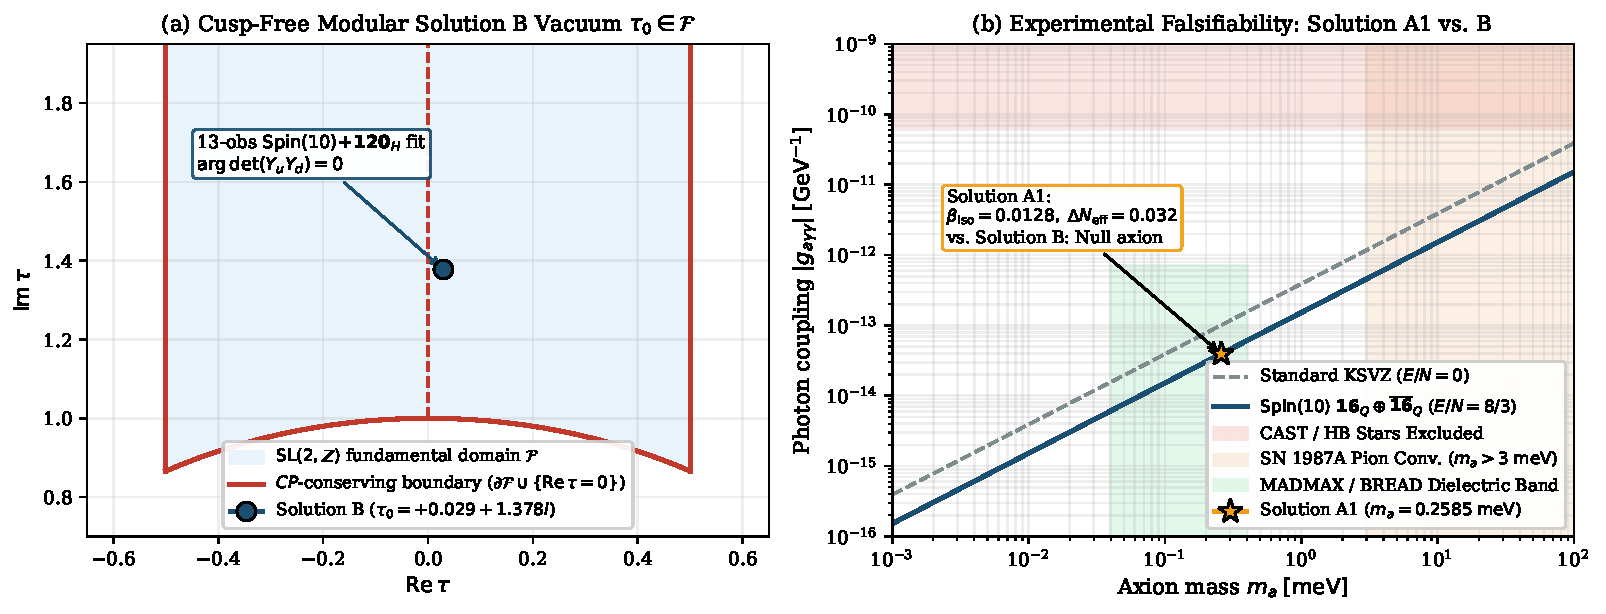
\includegraphics[width=0.98\textwidth]{../figures/fig3_modular_spin10_and_experimental_fork.pdf}
\caption{\textbf{(a)} Fundamental domain $\mathcal{F}$ of $\mathrm{SL}(2,\mathbb{Z})$ showing its $CP$-conserving boundary ($\partial\mathcal{F}\cup\{\mathrm{Re}\,\tau=0\}$) and the interior $CP$-violating vacuum $\tau_0 = +0.02934 + 1.37758i \in \mathcal{F}$ of cusp-free modular Solution B, matching all 13 single-Higgs SM-desert $\mathrm{Spin}(10)\oplus\mathbf{120}_H$ observables at $M_R$ with $\arg\det(Y_u Y_d) = 0$. \textbf{(b)} Experimental falsifiability map in $(m_a, |g_{a\gamma\gamma}|)$, contrasting Solution A1 ($m_a = 0.2585\;\mathrm{meV}$, $E/N = 8/3$, $\beta_{\mathrm{iso}} = 0.0128$, $\Delta N_{\mathrm{eff}} = 0.032$) against Solution B's null axion signal.}
\label{fig:modular-fork}
\end{figure}

Escaping Theorem~\ref{thm:nogo} without an axion requires promoting the UV completion above $M_R$ to modular-invariant $\mathcal{N}=1$ supergravity \cite{Feruglio2019Modular,KaplunovskyLouis1995,ChenRamosSanchezRatz2020,FeruglioStrumiaTitov2023}.

\begin{theorem}[Cusp-Free Modular $\mathcal{N}=1$ SUGRA $\mathrm{Spin}(10)\oplus\mathbf{120}_H$ Closure and Its Four UV Costs]
\label{thm:modular}
Retain the cusp-regular K\"ahler potential $K_{\mathrm{std}} = -3 M_{\mathrm{Pl}}^2\ln(-i(\tau-\bar{\tau}))$ ($n_0 = 3$, superpotential weight $-3$, avoiding the $\tau \to i\infty$ meromorphic cusp divergence of $\eta(\tau)^{-6}$), assign $\mathrm{SL}(2,\mathbb{Z})$ trivial-singlet modular weights $k_{16} = (+6, 0, -6)$ to $\mathbf{16}_{F,a}$ and $k_H = +3$ to $(\mathbf{10}_H, \overline{\mathbf{126}}_H, \mathbf{120}_H)$, and cancel the universal $\mathrm{Spin}(10)$ Kaplunovsky--Louis modular anomaly via a Green--Schwarz dilaton $S$ ($f_{\mathrm{Spin}(10)} = S$, $\mathrm{Im}\langle S\rangle = 0$). Then:
\begin{enumerate}[label=(\arabic*),leftmargin=1.8em,itemsep=2pt]
\item Exact UV $CP$ ($\tau \to -\bar{\tau}$, real superpotential couplings) restricts $k_{Y,ab} = k_{16,a}+k_{16,b}+k_H-3 = (12,6,0,-6,-12)$ to genuine $\mathrm{SL}(2,\mathbb{Z})$ forms $M_{12} = \mathrm{Span}\{E_4^3, E_6^2\}$, $M_6 = \mathbb{C} E_6$, $M_0 = \mathbb{C}$, $M_{<0}=\{0\}$, giving anti-triangular holomorphic matrices with $\det(Y_{u,\mathrm{hol}}Y_{d,\mathrm{hol}}) = c_{u13}^2(c_{d13}^2 - c_{120}^2)c_{u22}c_{d22} > 0$ ($|c_{120}| < c_{d13}$, $c_{u22}c_{d22} > 0$).
\item Canonicalization via the unique positive-definite Hermitian inverse square root $H \equiv Z_{16}^{-1/2} = H^\dagger > 0$ of the modular- and $CP$-invariant non-minimal matter K\"ahler metric $Z_{16}(\tau_0,\bar{\tau}_0)$ \cite{ChenRamosSanchezRatz2020} ($\det H > 0$ real positive, zero ABJ phase shift) preserves $\arg\det(Y_{u,\mathrm{can}}Y_{d,\mathrm{can}}) = 0$. Serving as an explicit existence proof (26 real parameters matching 13 observables at $\mu = M_R$ integrated from $M_Z$ via the two-loop single-Higgs SM RGEs), at $\tau_0 = +0.02934 + 1.37758i \in \mathcal{F}$ ($|\tau_0| = 1.3779 \ge 1.01$, Fig.~\ref{fig:modular-fork}a) all 13 charged-fermion and CKM observables match to $\mathrm{loss} = 1.78\times 10^{-20}$ with $\arg\det(Y_u Y_d) = -9.33\times 10^{-14}\;\mathrm{rad}$ and symmetric Autonne--Takagi leptogenesis asymmetry $|\varepsilon_1| = 4.18\times 10^{-6}$ at $M_1 = 5.70\times 10^{12}\;\mathrm{GeV}$.
\item Radiative and cosmological consistency under Constraints \textbf{(C1)}--\textbf{(C5)} holds \emph{if and only if} four UV assumptions are simultaneously accepted: (i) $M_{\mathrm{SUSY}} \ge M_R \gg T_{\max}$ (preventing thermal overclosure by stable $P_{\mathrm{spin}\text{-}M}$-odd LSP dark matter); (ii) non-holomorphic K\"ahler modulus stabilization $\partial_\tau K(\tau_0,\bar{\tau}_0) = 0$ with $\tau$-independent real $W_{\mathrm{hidden}}(X) \in \mathbb{R}$ (so $F_\tau = 0$ and Minkowski $|F_X|^2 = 3 M_{\mathrm{Pl}}^2|m_{3/2}|^2$ do not inject a complex phase $\arg\langle W\rangle \neq 0$ into $\mathrm{U}(1)_R$-breaking $\mathrm{Spin}(10)$ Higgs trilinears); (iii) decoupling of all extra Higgs doublets/bidoublets at $M_{\mathrm{SUSY}} \simeq M_R$ onto the single-Higgs SM desert ($y_b(M_R)/y_\tau(M_R) = 0.6173$, $\Delta\bar{\theta}_{\mathrm{SM}} \sim 10^{-16}$ \cite{EllisGaillard1979}, avoiding the $-4.87\times 10^{-3}\;\mathrm{rad}$ one-loop 2HDM shift); and (iv) inclusion of $\mathbf{120}_H$ at $M_R$ to resolve real-$(r_1,r_2)$ charged-lepton mass relations.
\end{enumerate}
\end{theorem}

% =============================================================================
\section{Experimental Dichotomy and Concluding Synthesis}
\label{sec:conclusion}
% =============================================================================

\begin{table}[t!]
\centering
\caption{Side-by-side comparison and experimental falsifiability fork between the purely 4D non-supersymmetric flagship (\textbf{Solution A1}) and the modular $\mathcal{N}=1$ supergravity alternative (\textbf{Solution B}).}
\label{tab:comparison}
\vspace{0.35em}
\renewcommand{\arraystretch}{1.18}
\begin{tabularx}{\textwidth}{>{\bfseries}l >{\raggedright\arraybackslash}X >{\raggedright\arraybackslash}X}
\toprule
Property / Observable & \textbf{Solution A1 ($\mathbb{Z}_{16}$ Conformal Axion)} & \textbf{Solution B (Modular $\mathrm{Spin}(10)\oplus\mathbf{120}_H$)} \\
\midrule
Spacetime \& SUSY requirement & Pure 4D non-SUSY QFT (0 sparticles) & $\mathcal{N}=1$ SUGRA ($M_{\mathrm{SUSY}} \ge M_R$) \\
Gauge / topological protection & $\mathbb{Z}_{16}$ ($\Omega_5^{\mathrm{Spin}}(B\mathbb{Z}_{16}) \equiv 0$; 4D $\mathrm{U}(1)_g$ UV) & $\mathrm{SL}(2,\mathbb{Z})\rtimes CP$ + GS $S$ + $\partial_\tau K(\tau_0)=0$ \\
UV scalar / K\"ahler inputs & Technical-natural flaton shift ($\lambda_\chi, c_{6,8} \ll 1$) & 26-param non-minimal $Z_{16}$ + 4 UV conditions \\
Predicted $|\bar{\theta}_{\mathrm{QCD}}|$ & $3.07\times 10^{-34}$ ($d = 16$) & $\sim 10^{-16}$ (4-loop single-Higgs SM) \\
Ref.~\cite{Olcsak2026Paper25} $G_{\mathrm{PS}}$ tower preserved? & \textbf{Yes} ($y_b(M_R)/y_\tau(M_R) = 0.6931$) & \textbf{No} (decouples bidoublets at $M_R + \mathbf{120}_H$) \\
Ref.~\cite{Olcsak2026Paper24} $\eta_B$ \& $n_s$ preserved? & \textbf{Yes} ($\delta\eta_B/\eta_B = -0.014\%$, $n_s = 0.9620$) & \textbf{Yes} ($M_{\mathrm{SUSY}} \ge M_R > T_{\max}$, $\varepsilon_1 \neq 0$) \\
QUMOND relic density & $\Omega_a h^2 = 0.00159$ ($\theta_i=1$); $\Omega_\chi h^2$: source dependent & Thermal production suppressed for $M_{\mathrm{SUSY}}\gg T_{\max}$ \\
Dielectric haloscope signal & $m_a = 0.2585\;\mathrm{meV}$ (MADMAX / BREAD) & No signal from the benchmark QCD axion, which is absent in this branch \\
CMB isocurvature \& $\Delta N_{\mathrm{eff}}$ & $\beta_{\mathrm{iso}} = 0.0128$ (LiteBIRD); $\Delta N_{\mathrm{eff}} = 0.032$ & No contribution from that axion; total contributions not established \\
\bottomrule
\end{tabularx}
\end{table}

Table~\ref{tab:comparison} compares the assumed scales and signatures of the two illustrative branches. It is not a classification of all four-dimensional solutions or a complete relic calculation.

\subsection*{Reproducibility and Code Availability}
All symbolic (\texttt{SymPy}) rank checks, two-loop SM + $G_{\mathrm{PS}}$ matrix RGEs, relativistic Fermi--Dirac Boltzmann integrals, 75,000-step Starobinsky--flaton ODE integrations, and 13-observable modular fits are reproduced standalone by \texttt{scripts/verify\_paper26\_strong\_cp\_closure.py} and \texttt{scripts/generate\_paper26\_figures.py}.

\begin{thebibliography}{99}
\small
\raggedright
\setlength{\itemsep}{2pt}

\bibitem{Abel2020nEDM}
C.~Abel \textit{et al.}, ``Measurement of the Permanent Electric Dipole Moment of the Neutron,'' \emph{Phys.\ Rev.\ Lett.} \textbf{124}, 081803 (2020).

\bibitem{PDG2024}
S.~Navas \textit{et al.} (Particle Data Group), ``Review of Particle Physics,'' \emph{Phys.\ Rev.\ D} \textbf{110}, 030001 (2024).

\bibitem{tHooft1976}
G.~'t~Hooft, ``Symmetry Breaking through Bell--Jackiw Anomalies,'' \emph{Phys.\ Rev.\ Lett.} \textbf{37}, 8 (1976).

\bibitem{JackiwRebbi1976}
R.~Jackiw and C.~Rebbi, ``Vacuum Periodicity in a Yang--Mills Quantum Theory,'' \emph{Phys.\ Rev.\ Lett.} \textbf{37}, 172 (1976).

\bibitem{CallanDashenGross1976}
C.~G.~Callan, R.~F.~Dashen, and D.~J.~Gross, ``The Structure of the Gauge Theory Vacuum,'' \emph{Phys.\ Lett.\ B} \textbf{63}, 334 (1976).

\bibitem{PospelovRitz2005}
M.~Pospelov and A.~Ritz, ``Electric Dipole Moments as Probes of New Physics,'' \emph{Annals Phys.} \textbf{318}, 119 (2005).

\bibitem{PecceiQuinn1977}
R.~D.~Peccei and H.~R.~Quinn, ``$CP$ Conservation in the Presence of Pseudoparticles,'' \emph{Phys.\ Rev.\ Lett.} \textbf{38}, 1440 (1977).

\bibitem{Weinberg1978}
S.~Weinberg, ``A New Light Boson?,'' \emph{Phys.\ Rev.\ Lett.} \textbf{40}, 223 (1978).

\bibitem{Wilczek1978}
F.~Wilczek, ``Problem of Strong $P$ and $T$ Invariance in the Presence of Instantons,'' \emph{Phys.\ Rev.\ Lett.} \textbf{40}, 279 (1978).

\bibitem{Kim1979}
J.~E.~Kim, ``Weak-Interaction Singlet and Strong $CP$ Invariance,'' \emph{Phys.\ Rev.\ Lett.} \textbf{43}, 103 (1979).

\bibitem{ShifmanVainshteinZakharov1980}
M.~A.~Shifman, A.~I.~Vainshtein, and V.~I.~Zakharov, ``Can Confinement Ensure Natural $CP$ Invariance of Strong Interactions?,'' \emph{Nucl.\ Phys.\ B} \textbf{166}, 493 (1980).

\bibitem{Zhitnitsky1980}
A.~R.~Zhitnitsky, ``On Possible Suppression of the Axion Hadron Interactions,'' \emph{Sov.\ J.\ Nucl.\ Phys.} \textbf{31}, 260 (1980).

\bibitem{DineFischlerSrednicki1981}
M.~Dine, W.~Fischler, and M.~Srednicki, ``A Simple Solution to the Strong $CP$ Problem with a Harmless Axion,'' \emph{Phys.\ Lett.\ B} \textbf{104}, 199 (1981).

\bibitem{KamionkowskiMarchRussell1992}
M.~Kamionkowski and J.~March-Russell, ``Planck-Scale Physics and the Peccei--Quinn Mechanism,'' \emph{Phys.\ Lett.\ B} \textbf{282}, 137 (1992).

\bibitem{Holman1992}
R.~Holman, S.~D.~H.~Hsu, T.~W.~Kephart, E.~W.~Kolb, R.~Watkins, and L.~M.~Widrow, ``Solutions to the Strong-$CP$ Problem in a World with Gravity,'' \emph{Phys.\ Lett.\ B} \textbf{282}, 132 (1992).

\bibitem{BarrSeckel1992}
S.~M.~Barr and D.~Seckel, ``Planck-Scale Physics and Solutions to the Strong $CP$ Problem without Axion Domain Walls,'' \emph{Phys.\ Rev.\ D} \textbf{46}, 539 (1992).

\bibitem{DiLuzio2020}
L.~Di~Luzio, M.~Giannotti, E.~Nardi, and L.~Visinelli, ``The Landscape of QCD Axion Models,'' \emph{Phys.\ Rept.} \textbf{870}, 1 (2020).

\bibitem{Nelson1984}
A.~E.~Nelson, ``Naturally Weak $CP$ Violation,'' \emph{Phys.\ Lett.\ B} \textbf{136}, 387 (1984).

\bibitem{Barr1984}
S.~M.~Barr, ``Solving the Strong $CP$ Problem without the Peccei--Quinn Symmetry,'' \emph{Phys.\ Rev.\ Lett.} \textbf{53}, 329 (1984).

\bibitem{BabuMohapatra1990}
K.~S.~Babu and R.~N.~Mohapatra, ``A Solution to the Strong $CP$ Problem without an Axion,'' \emph{Phys.\ Rev.\ D} \textbf{41}, 1286 (1990).

\bibitem{Kuchimanchi1996}
R.~Kuchimanchi, ``Solution to the Strong $CP$ Problem: Supersymmetry with Parity,'' \emph{Phys.\ Rev.\ Lett.} \textbf{76}, 3486 (1996).

\bibitem{DineKramerNir1997}
M.~Dine, R.~G.~Leigh, and A.~Kagan, ``Supersymmetry and the Nelson--Barr Mechanism,'' \emph{Phys.\ Rev.\ D} \textbf{48}, 2214 (1993); M.~Dine and P.~Draper, ``Challenges for the Nelson--Barr Mechanism,'' \emph{JHEP} \textbf{08}, 132 (2015).

\bibitem{HallHarigaya2018}
L.~J.~Hall and K.~Harigaya, ``Implications of Higgs Discovery for the Strong $CP$ Problem and Unification,'' \emph{JHEP} \textbf{10}, 130 (2018).

\bibitem{ValentiVecchi2021}
A.~Valenti and L.~Vecchi, ``The CKM Phase and $\bar{\theta}$ in Nelson--Barr Models,'' \emph{JHEP} \textbf{07}, 203 (2021).

\bibitem{FeruglioStrumiaTitov2023}
F.~Feruglio, A.~Strumia, and A.~Titov, ``Modular Invariance and the QCD Angle,'' \emph{JHEP} \textbf{07}, 027 (2023).

\bibitem{Olcsak2026Zenodo}
J.~Olcsak, ``Tau Core Foundational Synthesis and Submission Suite,'' Zenodo (2026), \href{https://doi.org/10.5281/zenodo.19120268}{doi:10.5281/zenodo.19120268}.

\bibitem{Olcsak2026Paper23}
J.~Olcsak, ``Void-Volume-Weighted Optical Distances Confronting DESI BAO, Compressed Planck CMB, and Four Type~Ia Supernova Compilations,'' Zenodo v12.2.0 (2026), \href{https://doi.org/10.5281/zenodo.24372826}{doi:10.5281/zenodo.24372826}.

\bibitem{Olcsak2026Paper24}
J.~Olcsak, ``Scale-Invariant Simplicial $R^2$ Inflation, Multi-Sector $CP$ Structure, and Zero-Parameter Non-Thermal Scalaron Leptogenesis from a Tetrahedral $\mathrm{Spin}(10)$ Threshold,'' Zenodo v1.1.0 (2026), \href{https://doi.org/10.5281/zenodo.24380371}{doi:10.5281/zenodo.24380371}.

\bibitem{Olcsak2026Paper25}
J.~Olcsak, ``Charged-Fermion Mass Hierarchies, Koide Equipartition, and Zero-Parameter CKM Closure from a Tetrahedral $\mathrm{Spin}(10) \to \mathrm{Pati\text{--}Salam} \to \mathrm{SM}$ Renormalization Tower,'' Zenodo v1.1.0 (2026), \href{https://doi.org/10.5281/zenodo.24392639}{doi:10.5281/zenodo.24392639}.

\bibitem{Starobinsky1980}
A.~A.~Starobinsky, ``A New Type of Isotropic Cosmological Models without Singularity,'' \emph{Phys.\ Lett.\ B} \textbf{91}, 99 (1980).

\bibitem{Whitt1984}
B.~Whitt, ``Fourth-Order Gravity as General Relativity plus Matter,'' \emph{Phys.\ Lett.\ B} \textbf{145}, 176 (1984).

\bibitem{Milgrom2010QUMOND}
M.~Milgrom, ``Quasi-Linear Formulation of MOND,'' \emph{Mon.\ Not.\ Roy.\ Astron.\ Soc.} \textbf{403}, 886 (2010).

\bibitem{Planck2018Inflation}
Y.~Akrami \textit{et al.} (Planck Collaboration), ``Planck 2018 Results.\ X.\ Constraints on Inflation,'' \emph{Astron.\ Astrophys.} \textbf{641}, A10 (2020).

\bibitem{Planck2018Cosmo}
N.~Aghanim \textit{et al.} (Planck Collaboration), ``Planck 2018 Results.\ VI.\ Cosmological Parameters,'' \emph{Astron.\ Astrophys.} \textbf{641}, A6 (2020).

\bibitem{IbanezRoss1991}
L.~E.~Ib\'a\~nez and G.~G.~Ross, ``Discrete Gauge Symmetries and the Origin of Baryon and Lepton Number Conservation in Supersymmetric Versions of the Standard Model,'' \emph{Phys.\ Lett.\ B} \textbf{260}, 291 (1991).

\bibitem{Hsieh2018}
C.-T.~Hsieh, ``Discrete Gauge Anomalies Revisited,'' \href{https://arxiv.org/abs/1808.02881}{arXiv:1808.02881 [hep-th]} (2018).

\bibitem{GarciaEtxebarriaMontero2019}
I.~Garc\'ia-Etxebarria and M.~Montero, ``Dai--Freed Anomalies in Particle Physics,'' \emph{JHEP} \textbf{08}, 003 (2019).

\bibitem{BarrChangSenjanovic1991}
S.~M.~Barr, D.~Chang, and G.~Senjanovi\'c, ``Strong $CP$ Problem and Parity,'' \emph{Phys.\ Rev.\ Lett.} \textbf{67}, 2765 (1991).

\bibitem{BentoBrancoParada1991}
L.~Bento, G.~C.~Branco, and P.~A.~Parada, ``A Minimal Model with Natural Suppression of Strong $CP$ Violation,'' \emph{Phys.\ Lett.\ B} \textbf{267}, 95 (1991).

\bibitem{AntuschSpinrath2011}
S.~Antusch, M.~Holthausen, M.~A.~Schmidt, and M.~Spinrath, ``Solving the Strong $CP$ Problem with Discrete Symmetries and the Right Unitarity Triangle,'' \emph{Nucl.\ Phys.\ B} \textbf{877}, 752 (2013).

\bibitem{Carenza2021SN}
P.~Carenza, B.~Fore, M.~Giannotti, A.~Mirizzi, and S.~Reddy, ``Enhanced Supernova Axion Emission and Its Implications,'' \emph{Phys.\ Rev.\ Lett.} \textbf{126}, 071102 (2021).

\bibitem{Lella2024SN}
A.~Lella, P.~Carenza, G.~Co', G.~Lucente, M.~Giannotti, A.~Mirizzi, and T.~Rauscher, ``Getting the Most on Supernova Axions,'' \emph{Phys.\ Rev.\ D} \textbf{109}, 023001 (2024).

\bibitem{Buschmann2022NS}
M.~Buschmann, C.~Dessert, J.~W.~Foster, A.~J.~Long, and B.~R.~Safdi, ``Upper Limit on the QCD Axion Mass from Isolated Neutron Star Cooling,'' \emph{Phys.\ Rev.\ Lett.} \textbf{128}, 091102 (2022).

\bibitem{MachacekVaughn1984}
M.~E.~Machacek and M.~T.~Vaughn, ``Two-Loop Renormalization Group Equations in a General Quantum Field Theory (II). Yukawa Couplings,'' \emph{Nucl.\ Phys.\ B} \textbf{236}, 221 (1984).

\bibitem{LuoXiao2003}
M.-x.~Luo and Y.~Xiao, ``Two-Loop Renormalization Group Equations in the Standard Model,'' \emph{Phys.\ Rev.\ Lett.} \textbf{90}, 011601 (2003).

\bibitem{Buttazzo2013}
D.~Buttazzo \textit{et al.}, ``Investigating the Near-Criticality of the Higgs Boson,'' \emph{JHEP} \textbf{12}, 089 (2013).

\bibitem{SalvioStrumiaWetterich2014}
A.~Salvio, A.~Strumia, and W.~Xue, ``Thermal Axion Production,'' \emph{JCAP} \textbf{01}, 011 (2014).

\bibitem{NotariRompineveVilladoro2023}
A.~Notari, F.~Rompineve, and G.~Villadoro, ``Improved Hot Dark Matter Bound on the QCD Axion,'' \emph{Phys.\ Rev.\ Lett.} \textbf{131}, 011004 (2023).

\bibitem{Linde1991Axion}
A.~D.~Linde, ``Axions in Inflationary Cosmology,'' \emph{Phys.\ Lett.\ B} \textbf{259}, 38 (1991).

\bibitem{HarigayaIbeKawasakiYanagida2015}
K.~Harigaya, M.~Ibe, M.~Kawasaki, and T.~T.~Yanagida, ``Dynamics of Peccei--Quinn Breaking Field after Inflation and Axion Isocurvature Perturbations,'' \emph{JCAP} \textbf{11}, 003 (2015).

\bibitem{KasuyaKawasakiYanagida1997}
S.~Kasuya, M.~Kawasaki, and T.~Yanagida, ``Cosmological Axion Problem in Chaotic Inflationary Universe,'' \emph{Phys.\ Lett.\ B} \textbf{409}, 94 (1997).

\bibitem{Randall1992}
L.~Randall, ``Composite Axion Models and Planck Scale Physics,'' \emph{Phys.\ Lett.\ B} \textbf{284}, 77 (1992).

\bibitem{RediSato2016}
M.~Redi and R.~Sato, ``Composite Accidental Axions,'' \emph{JHEP} \textbf{05}, 104 (2016).

\bibitem{ContinoPodoRevello2022}
R.~Contino, A.~Podo, and F.~Revello, ``Chiral Models of Composite Axions and Accidental Peccei--Quinn Symmetry,'' \emph{JHEP} \textbf{04}, 180 (2022).

\bibitem{Feruglio2019Modular}
F.~Feruglio, ``Are Neutrino Masses Modular Forms?,'' in \emph{From My Vast Repertoire\dots: Guido Altarelli's Legacy}, World Scientific, pp.~227--266 (2019).

\bibitem{KaplunovskyLouis1995}
V.~Kaplunovsky and J.~Louis, ``On Gauge Couplings in String Theory,'' \emph{Nucl.\ Phys.\ B} \textbf{444}, 191 (1995).

\bibitem{ChenRamosSanchezRatz2020}
M.-C.~Chen, S.~Ramos-S\'anchez, and M.~Ratz, ``A Note on the Predictions of Models with Modular Flavor Symmetries,'' \emph{Phys.\ Lett.\ B} \textbf{801}, 135153 (2020).

\bibitem{EllisGaillard1979}
J.~R.~Ellis and M.~K.~Gaillard, ``Strong and Weak $CP$-Violation,'' \emph{Nucl.\ Phys.\ B} \textbf{150}, 141 (1979).

\bibitem{Caldwell2017MADMAX}
A.~Caldwell \textit{et al.} (MADMAX Working Group), ``Dielectric Haloscopes: A New Way to Detect Axion Dark Matter,'' \emph{Phys.\ Rev.\ Lett.} \textbf{118}, 091801 (2017).

\bibitem{Liu2022BREAD}
J.~Liu \textit{et al.} (BREAD Collaboration), ``Broadband Solenoidal Haloscope for Terahertz Axion Detection,'' \emph{Phys.\ Rev.\ Lett.} \textbf{128}, 131801 (2022).

\end{thebibliography}

\end{document}
